\chapter{光栅化}

\textbf{Keyword. } \textsl{重心坐标}

\hspace*{1em}

虎书中有这么一段话: The process of finding all the pixels in an image that are occupied by a geometric primitive is called rasterization; 即光栅化就是找到所有被几何原型所占据的所有像素点(找到这些像素点之后再进行逐个渲染)。其中三角形就是最常用的geometric primitive

\section{线性插值}

二维或者三维的情况,插入一个位置形成线段,由$a,b$两点构成以$t$为参数的直线性质\footnote{这是一个0单纯形},
\begin{equation}
    p=(1-t)a+tb
\end{equation}

这就是插值,因为系数$t$和$1-t$是$t$的线性多项式,所以称为\textsl{线性插值}。

另一种线性插值的情况,对于$x$轴上一组点,$x_1,x_2,\cdots,x_n$,我们想建立一个连续函数$y=f(x)$来插入这些点。
,使得$f$能通过每一个数据点,即$f(x_i)=y_i$。在线性插值中,各点$(x_i,y_i)$由直线相连。
\begin{equation}
    f(x)=y_i+\frac{x-x_i}{x_{i+1}-x_i}(y_{i+1}-y_i)
\end{equation}

\section{重心坐标}

数学中,重心坐标是由单形(如三角形或四面体等)顶点定义的坐标。重心坐标是齐次坐标的一种。

设$v1,\cdots,vn$是向量空间V中一个单形的顶点,如果$V$中某点$p$满足
\begin{equation}
    (\lambda_1+\lambda_2+\cdots+\lambda_n)p=\lambda_1v_1+\lambda_2v_2+\cdots+\lambda_nv_n
\end{equation}

那么我们称系数$(\lambda_1,\cdots, \lambda_n)$是$ p$关于$v_1,\cdots,v_n$的重心坐标。

重心坐标不是惟一的:对任何不等于零的$k$,$(k\lambda_1,\cdots, k\lambda_n)$也是p的重心坐标。但总可以取坐标满足 $\lambda_1+\cdots+\lambda_n = 1$,称为\textsl{正规化坐标}。注意到定义式在仿射变换下不变,故重心坐标具有仿射不变性。 

\subsection*{三角形的重心坐标}

在三角形情形中,重心坐标也叫面积坐标,因为P点关于三角形ABC的重心坐标和三角形PBC, PCA及PAB的(有向)面积成比例

\begin{figure}[H]
    \centering
    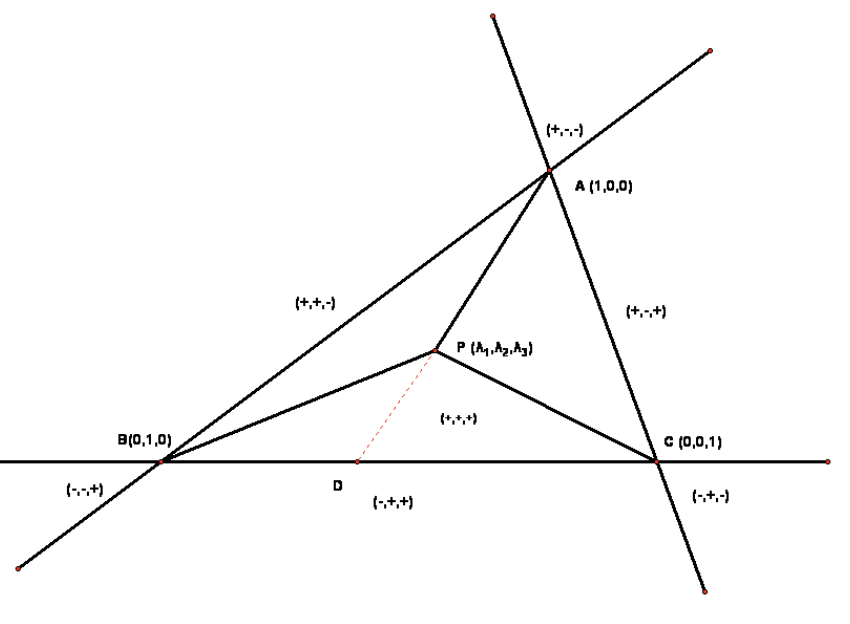
\includegraphics[scale=0.35]{figures/三角形重心坐标.png}
    \caption{三角形重心坐标}
\end{figure}

\subsection*{笛卡尔坐标系中的三角形面积}

数学中常常用向量之间的“矩”来量化几何体的面积。考虑三角形ABC的面积
\begin{equation}
    S=\frac{1}{2}\Vert\overrightarrow{AB}\times\overrightarrow{AC}\Vert
\end{equation}

其中$\overrightarrow{AB}=(x_1,x_2,x_3)$,$\overrightarrow{AC}=(y_1,y_2,y_3)$表示成行列式
\begin{equation}
    S=\frac{1}{2}\Vert\left|
        \begin{array}{ccc}
            i   &   j   & k  \\
            x_1 &  x_2  & x_3\\
            y_1 &  y_2  & y_3\\
        \end{array}
    \right|\Vert
\end{equation}

即

\begin{equation}
    S=\frac{1}{2}\left|
        \begin{array}{ccc}
            1   &   1   & 1  \\
            x_1 &  x_2  & x_3\\
            y_1 &  y_2  & y_3\\
        \end{array}
    \right|
\end{equation}

\subsection*{重心坐标系}

重心坐标系是一种仿射坐标系,在图形学中,经常希望为三角形的每个顶点赋予性质,如颜色,并将该性质的值插值到三角形中,实现这种要求
的方法是利用\textsl{重心坐标系}

\begin{figure}[H]
    \centering
    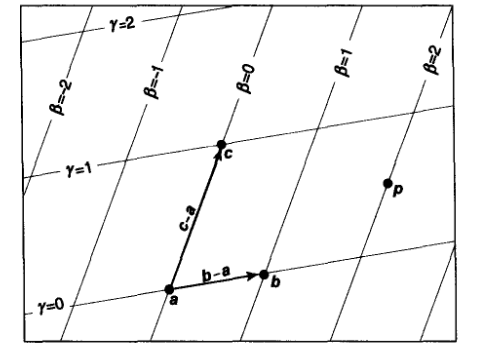
\includegraphics[scale=0.35]{figures/重心坐标系.png}
    \caption{重心坐标系}
\end{figure}

如上图所示,期坐标原点为$a$,从$a$到$b$和$c$的向量为基向量。于是$p$点就可以表示成
\begin{equation}
    p=a+\beta(b-a)+\gamma(c-a)
\end{equation}

重新安排顺序
\begin{equation}
    p=(1-\beta-\gamma)a+b+c
\end{equation}

令$\alpha=1-\beta-\gamma$,于是得到方程
\begin{equation}
    p=\alpha a+\beta b+\gamma c
\end{equation}

其中$\alpha+\beta+\gamma=1$。

重心坐标系的一大特点是,对于由$a,b,c$形成的三角形,当且仅当下列条件满足时,点$p$位于三角形内部
\begin{equation}
    \begin{aligned}
        & 0<\alpha<1\\
        & 0<\beta<1\\
        & 0<\gamma<1\\
    \end{aligned}
\end{equation}

\section{直线的光栅化}

基于隐式方程绘制直线的常用算法是\textsl{中点算法}。直线的一般方程是
\begin{equation}
    f(x,y)=(y_0-y_1)x+(x_1-x_0)y+x_0y_1-x_1y_0=0
\end{equation}

我们先来考虑直线斜率$k\in(0,1)$的情况。在这种情况下,直线是以沿$x$轴方向的变化要快于沿$y$轴方向的变化。此时的直线是一条从左向右平缓上升的直线。
不难想象的是,这时我们要光栅化一条直线的话,从左下角的起点出发,每次要“点亮”的像素的 
$x$坐标都是上一个像素的$x$坐标加1,而$y$坐标则是根据某种条件,保持不变或者加1,如此反复直至终点。

现在的关键就在于条件是什么?那么中点算法就是来解决这个问题的。

\subsection*{中点算法}

中点算法的核心内容是:当我们要确定下一个要“点亮”的像素时,我们就把位于右侧和右上侧的这两个待选择的像素中心点的中点带入到直线方程中去,根据这个中点
位于该直线的上侧还是下侧来决定“点亮”右侧的像素还是右上侧的像素。在保证$y$是正系数的情况下\footnote{如果$y$不是正系数,则情况相反,例如$f(x,y)=x-y+1$,点$f(0,0)=1>0$但是位于直线下方},如果中点位于直线上方,则$f(x,y)>0$,如果中点位于下方,则$f(x,y)<0$。

\begin{figure}[H]
    \centering
    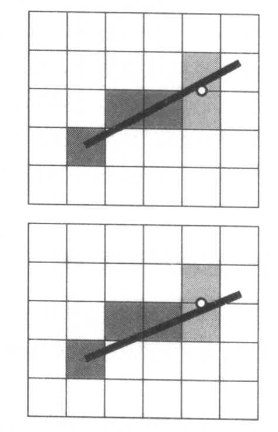
\includegraphics[scale=0.5]{figures/中点算法的两种情况.png}
    \caption{中点算法的两种情况}
\end{figure}

\subsection*{证明}

\begin{proposition}
    在保证$y$是正系数的情况下\footnote{如果$y$不是正系数,则情况相反,例如$f(x,y)=x-y+1$,点$f(0,0)=1>0$但是位于直线下方},如果中点位于直线上方,则$f(x,y)>0$,如果中点位于下方,则$f(x,y)<0$。
\end{proposition}

\textbf{proof. } 直线的参数方程为
\begin{equation}
    t=\frac{x-x_0}{a}=\frac{y-y_0}{b}=\frac{z-z_0}{c}
\end{equation}

其中$(a,b,c)$是和直线平行的一个向量。要证明

\subsection*{中点算法的改进—Bresenham算法}

中点算法有个很大的弊端就是每循环一次就要将中点带入方程求解并判断一次。我们有必要每次都求解方程吗?能不能只求解一次方程就可以呢?这就引入了中点算法的增量形式—Bresenham算法。

因为中点算法首先是将两个像素点中点代入方程,然后计算出$f(x,y)$的正负,但是我们发现,\textsl{中点之间的增量都是固定的},这意味着我们只要求出来一个中点相对直线的位置,下一个
中点的位置只需要加上固定增量即可。增量存在如下关系
\begin{equation}
    \begin{aligned}
        & f(x+1,y)=f(x,y)+(y-y_0) \\
        & f(x+1,y+1)=f(x,y)+(y-y_0)+(x-x_0)
    \end{aligned}
\end{equation}

\section{三角形光栅化}

v、为什么要以三角形的光栅化为例呢,因为三角形是最基本的多边形,大部分的模型都是用一个个三角形表示,任意的其它多边形其实都可以转化成多个三角形的形式。

如下图所示,如何将三角形绘制到屏幕上?

\begin{figure}[H]
    \centering
    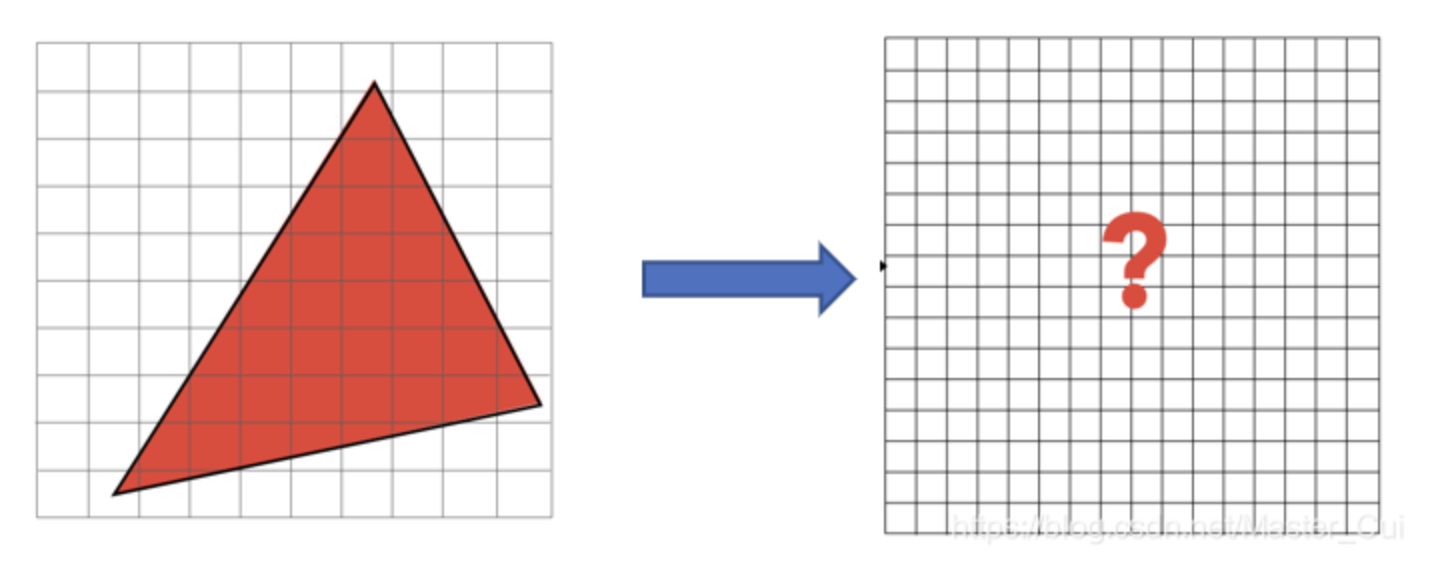
\includegraphics[scale=0.2]{figures/三角形光栅化.png}
    \caption{三角形光栅化}
\end{figure}

首先需要进行采样,采样的意思就是对给定的函数进行离散化,比如上图中,要实现一个判断屏幕上的像素是否在三角形内的函数,然后将三角形顶点构成的最大长方形区域内所有点作为函数的输入,判断这些点是否在三角形内,如果在三角形内,就将屏幕上的像素点进行点亮。这个过程就是采样。
其他采样的例子包括对视频进行时间上的采样,这样就可以得到视频中的某几帧画面

\subsection*{判断像素点是否在三角形内部}

利用同侧向量积可以判断像素点是否在三角形内部

\begin{figure}[H]
    \centering
    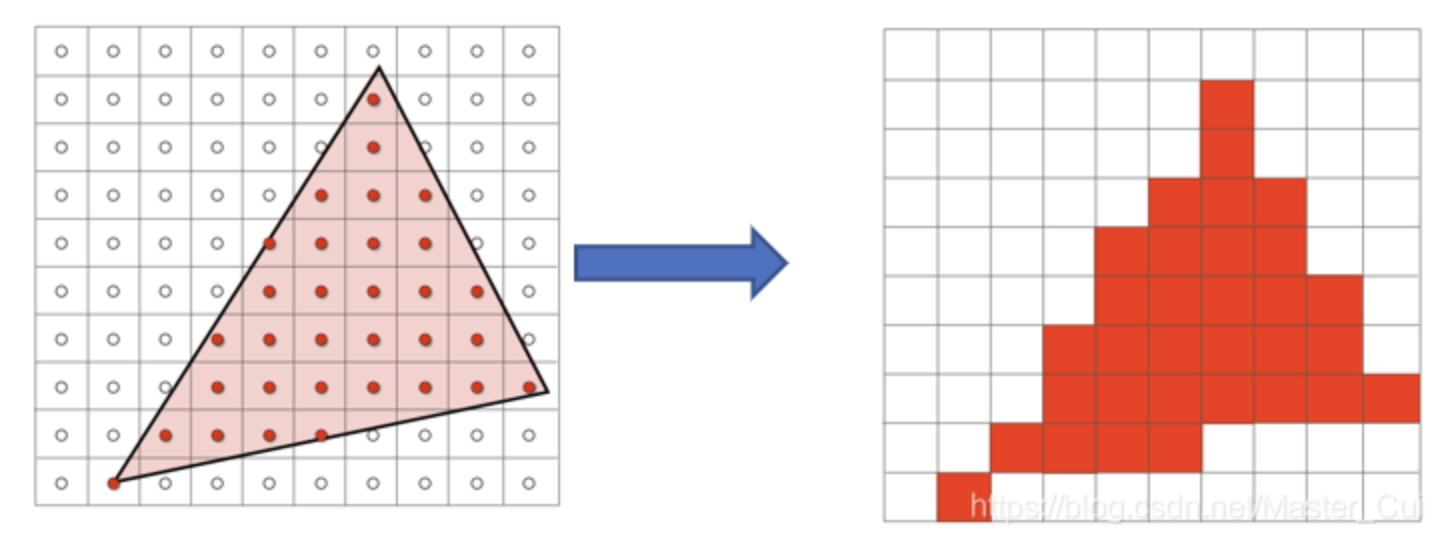
\includegraphics[scale=0.2]{figures/采样后的三角形.png}
    \caption{采样后的三角形}
\end{figure}

\section{反走样}

\subsection*{抗锯齿}

锯齿产生的原因就是因为信号的变化频率高,而相应的采样频率低。就三角形边缘不规则的情况来说,因为
三角形的边上是无限多个点,而用有限个方块去逼近无限多个点的三角形的边,所以当然会产生不规则的锯
齿,硬件的解决办法一是可以加大屏幕的分辨率,使得像素变小,从而可以得到更多个有限的方块去逼近三
角形。而软件的方法就是加入抗锯齿算法。无论是硬件方法还是软件方法,都不能完全解决锯齿问题,只能缓解锯齿问题,直到人眼察觉不出来

\begin{figure}[H]
    \centering
    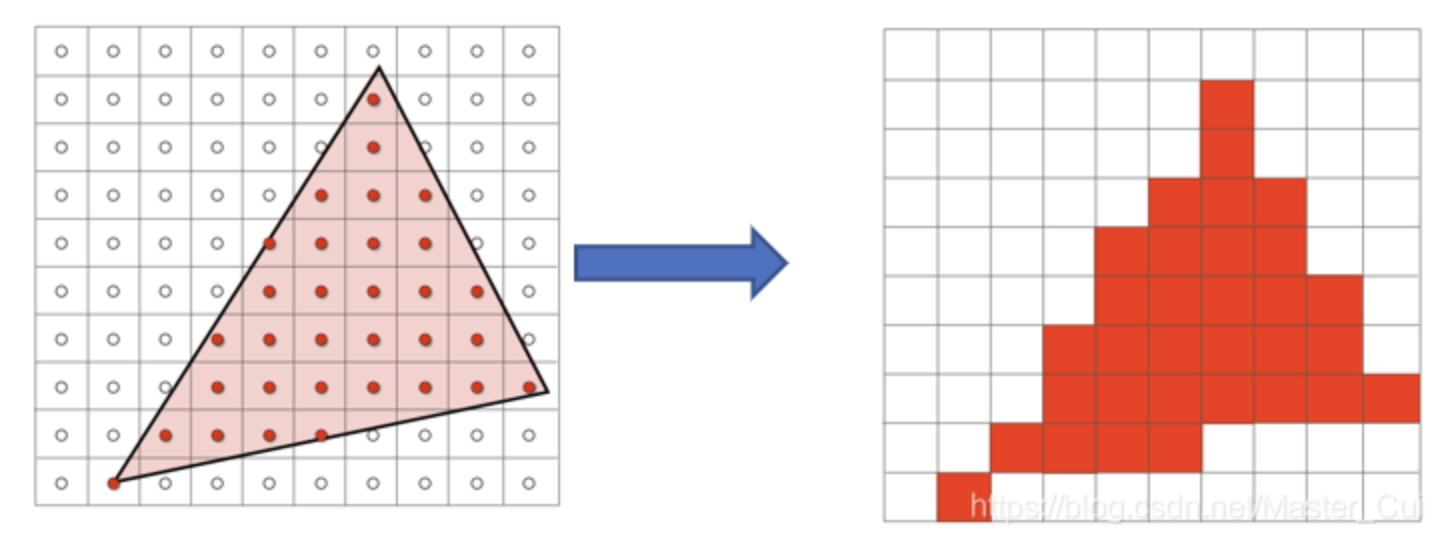
\includegraphics[scale=0.2]{figures/采样后的三角形.png}
    \caption{采样后的三角形}
\end{figure}

\subsection*{利用平滑算子进行模糊三角形边界}

平缓算子和图像卷积,在时域或频域进行。常用的平滑算子是计算邻域内的平均值。

\begin{figure}[H]
    \centering
    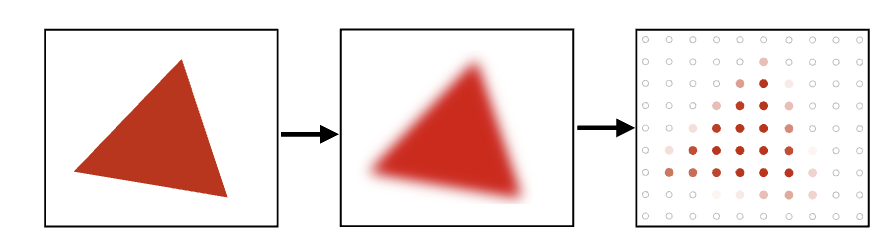
\includegraphics[scale=0.4]{figures/模糊算子.png}
    \caption{经过平滑算子之后在进行光栅化}
\end{figure}

\subsection*{SSAA(super sampling antialisa,超采样抗锯齿算法)}

它的原理非常简单,就是在渲染时将要输出的分辨率提升 x 倍,比如要输出 1920x1080 的分辨率到屏幕上,开启 SSAA 2x, 那么内部渲染时的分辨率就是 3840x2160, 然后 Downsampling 到 1920x1080 上,自然在许多纹理边缘上就显得平滑许多。

SSAA的思想就是将一个像素分解成2*2,3*3,4*4......,然后判断分解后像素中的4个或者9个或者16个像素点是否在三角形内,如果在像素内,就将点绘制成红色,然后将
这4个或者9个或者16个像素点的像素值求平均值,最后作为整个像素点的像素值。

例如一个2*2的过程

\begin{figure}[H]
    \centering
    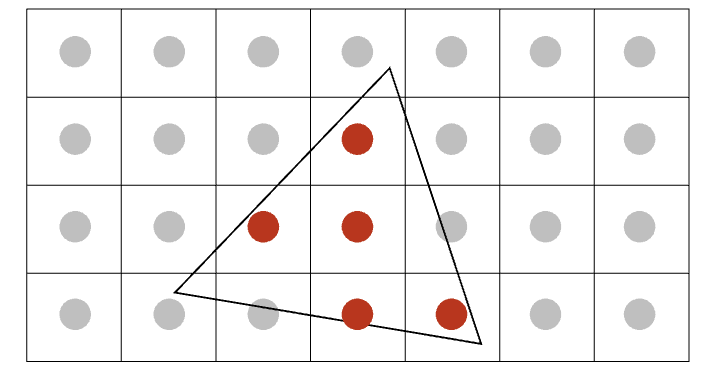
\includegraphics[scale=0.3]{figures/SSAA1.png}
    \caption{原始采样}
\end{figure}

\begin{figure}[H]
    \centering
    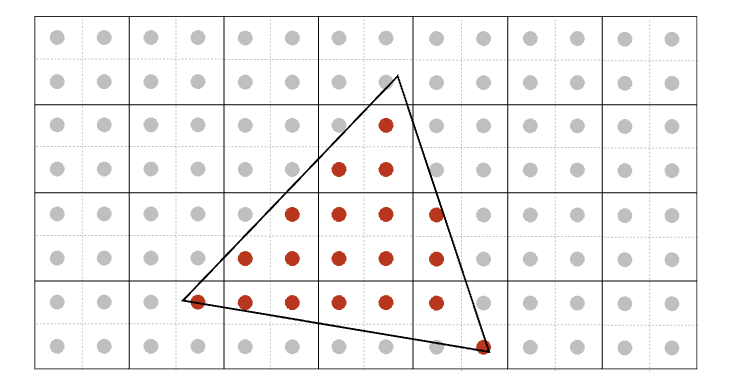
\includegraphics[scale=0.3]{figures/SSAA2.png}
    \caption{细分每个像素的子像素}
\end{figure}

如果子像素在三角形内部则赋予红色。

\begin{figure}[H]
    \centering
    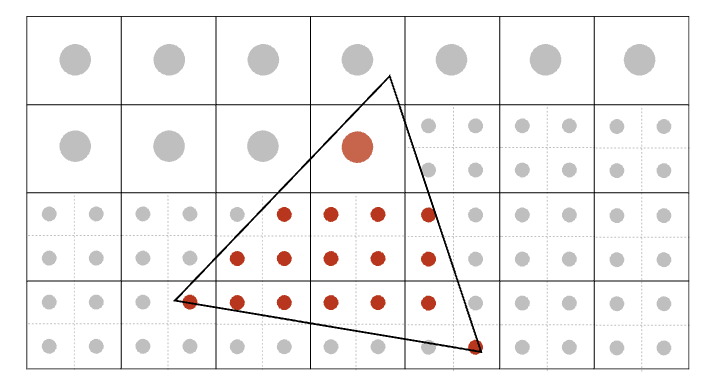
\includegraphics[scale=0.3]{figures/SSAA3.png}
    \caption{求大像素内每个小像素平均值}
\end{figure}

\begin{figure}[H]
    \centering
    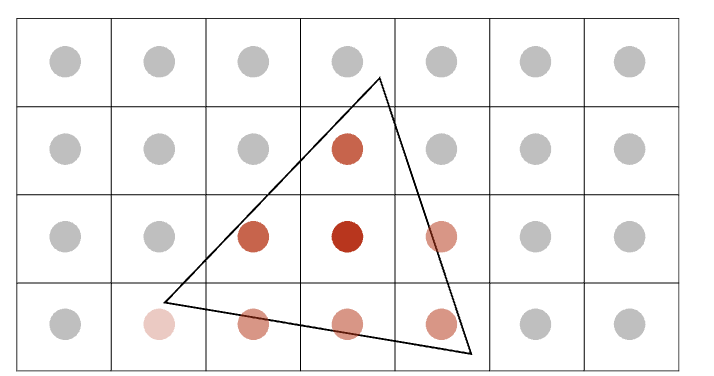
\includegraphics[scale=0.3]{figures/SSAA4.png}
    \caption{平均每个像素}
\end{figure}

\subsection*{MSAA(multi-sampling antialisa,多采样抗锯齿算法)}

MSAA 只对于多边形的边缘进行抗锯齿处理。比如一个红色的圆,只对圆周作抗锯齿多重采样计算,但是圆周以内的部分则不会处理。这种方式下的画面锯齿得到了一定的抑制,而抗锯齿需要的资源也大幅下降到可接受的范围中。所以 MSAA 也逐渐成为目前被使用的最多的抗锯齿技术。

MSAA的思想就是如果有子采样像素在三角形内,那么,就认为像素点需要着色,采样后,看有多少个子采样像素点在三角形内,然后计算在三角形内的子采样像素占所有采样点的比重,
最后把整体的像素值(比如红色)乘以该比重,就得到了最终绘制的像素值。

\section{对图形深度的处理}

\subsection*{画家算法}

画家算法”表示头脑简单的画家首先绘制距离较远的场景,然后用绘制距离较近的场景覆盖较远的部分。 画家算法首先将场景中的多边形根据深度进行排序,然后按照顺序进行描绘。 这种方法通常会将不可见的部分覆盖,这样就可以解决可见性问题。 
在有些场合下,画家算法可能无法解决可见性问题。例如下面重叠三角形

\begin{figure}[H]
    \centering
    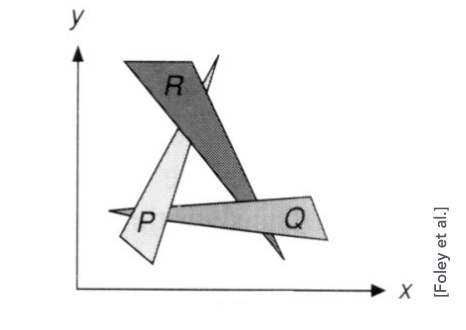
\includegraphics[scale=0.6]{figures/画家算法.png}
    \caption[short]{画家算法无法按照先后顺序表示图中重叠物体}
\end{figure}

\subsection*{深度缓冲算法(Z-Buffer)}

算法的过程是:

\begin{enumerate}[itemindent=2em]
    \item \textsl{首先分配一个数组buffer,数组的大小为像素的个数,数据中的每个数据都表示深度,初始深度值为无穷大}。
    \item \textsl{随后遍历每个三角形上的每个像素点[x,y],如果该像素点的深度值z<zbuffer[x,y]中的值,则更新zbuffer[x,y]值为该点深度值z,并更新该像素点[x,y]的颜色为该三角形上像素点上的颜色。}
\end{enumerate}

说白了就是每个像素点去对比深度,伪代码表示

\begin{lstlisting}[language=python]
    for(each triangle T)
        for(each sample point (x,y,z) in T)
            if(z<zbuffer[x,y])
                framebuffer[x,y]=rgb;
                zbuffer[x,y]=z;
            else
            ;
\end{lstlisting}

例如下面图,$R$表示无穷大,红色和紫色为需要绘制的三角形。
\begin{figure}[H]
    \centering
    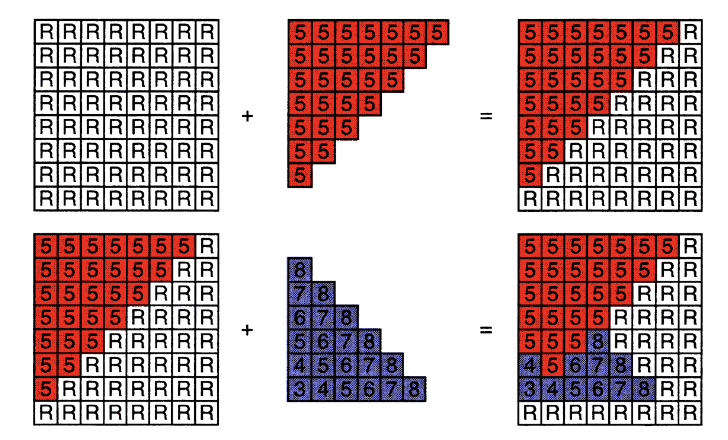
\includegraphics[scale=0.6]{figures/zbuffer.png}
    \caption[short]{zbuffer algorithm}
\end{figure}

